\documentclass{article}
\usepackage{graphicx} % new way of doing eps files
\usepackage{listings} % nice code layout
\usepackage[usenames]{color} % color
\definecolor{listinggray}{gray}{0.9}
\definecolor{graphgray}{gray}{0.7}
\definecolor{ans}{rgb}{1,0,0}
\definecolor{blue}{rgb}{0,0,1}
% \Verilog{title}{label}{file}
\newcommand{\Verilog}[3]{
  \lstset{language=Verilog}
  \lstset{backgroundcolor=\color{listinggray},rulecolor=\color{blue}}
  \lstset{linewidth=\textwidth}
  \lstset{commentstyle=\textit, stringstyle=\upshape,showspaces=false}
  \lstset{frame=tb}
  \lstinputlisting[caption={#1},label={#2}]{#3}
}


\author{Jon Johnston and Justin Roessler}
\title{Lab 2 - Program Counter}

\begin{document}
\maketitle

\section{Executive Summary}
The purpose of this lab was to make a 64-bit adder and a 64-bit mux. These modules will be implemented into our ARM processor. Also two test benches were created to test each module. The adder will update our Program Counter with each clock cycle and the mux will be used to set the Program Counter to the incremented PC or to a different address based on the control line. 

Also, this lab helped us regather our knowledge with verilog and git. Tasks such as creating a new file, resetting the top module ,and updating files were a good refresher on using these programs.

\section{Test Report}
To verify operation of these two modules, this lab requires two separate test benches.
\begin{enumerate}
	\item Adder Test Bench
	\item Mux Test Bench
\end{enumerate}

\subsection{Adder Test Bench}
The adder test bench contains:
\begin{enumerate}
	\item Inputs
	\begin{enumerate}
		\item A\_in - the first 64-bit number
		\item B\_in - the second 64-bit number
	\end{enumerate}	
	\item Outputs
	\begin{enumerate}	
		\item Add\_out - the 64-bit sum of the two input numbers
	\end{enumerate}
\end{enumerate} 
The adder test bench sets the values of two input numbers, a and b, and sends the numbers into the adder module. The adder module adds these two numbers together and gives us our result. Correct operation is verified by comparing the Simulation Results with the Expected Results Table.  After analyzing the results, the adder works as expected.

\begin{figure}
	\begin{center}
		\caption{Expected Results of the adder test.}\label{fig:ert_addertest}
		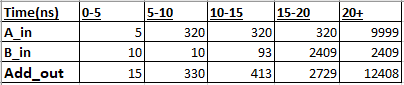
\includegraphics[width=1.0\textwidth]{../images/AdderExpected.png}
	\end{center}
\end{figure}

\begin{figure}
	\begin{center}
		\caption{Timing diagram for the adder test.}\label{fig:addertest}
		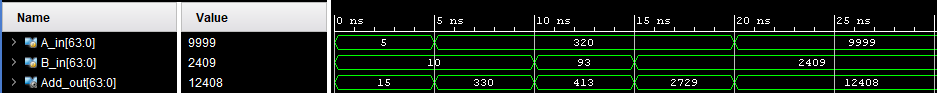
\includegraphics[width=1.0\textwidth]{../images/AdderSimulation.png}
	\end{center}
\end{figure}

\subsection{Mux Test Bench}
The mux test bench contains:
\begin{enumerate}
	\item Inputs
	\begin{enumerate}
		\item a\_in - the first 64-bit mux input, which is passed to mux\_out when the control line is set to 0 
		\item b\_in - the second 64-bit mux input, which is passed to mux\_out when the control line is set to 1
		\item control - the 1-bit control input to the mux which determines whether a or b will be passed to mux\_out
	\end{enumerate}	
	\item Outputs
	\begin{enumerate}	
		\item mux\_out - the 64-bit output of the mux
	\end{enumerate}
\end{enumerate} 

The mux\_test bench sets the values of a, b, and the control line and verifies that mux\_out is set to the correct value. The mux module takes the inputs and gives us a when control is 0 and b when control is 1. Based on 4 cases conducted in the mux\_test module, correct operation is verified by comparing the Simulation Results with the Expected Results Table.  After analyzing the results, the mux works as expected.

\begin{figure}
	\begin{center}
		\caption{Expected Results of the mux test.}\label{fig:ert_muxtest}
		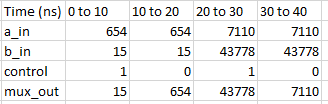
\includegraphics[width=1.0\textwidth]{../images/MuxExpected.png}
	\end{center}
\end{figure}

\begin{figure}
	\begin{center}
		\caption{Timing diagram for the mux test.}\label{fig:muxtest}
		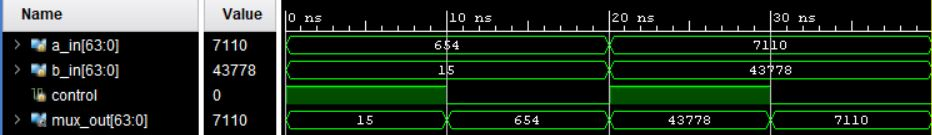
\includegraphics[width=1.0\textwidth]{../images/MuxSimulation.jpg}
	\end{center}
\end{figure}

\pagebreak

\section{Code Appendix}
\Verilog{Verilog code for testing the adder.}{code:addertest}{../code/0_common/adder_test.v}
\Verilog{Verilog code for the adder.}{code:adder}{../code/0_common/adder.v}
\Verilog{Verilog code for testing the mux.}{code:muxtest}{../code/0_common/mux_test.v}
\Verilog{Verilog code for the mux.}{code:mux}{../code/0_common/mux.v}

\end{document} 